\section{Implementation results}
\label{sec:results}

\subsection{Test performance and model size}
\label{sec:quantitative}
CNN achieves 92.59\% accuracy and a macro-F1 of 0.9261 on the official
Fashion-MNIST test set. It exceeds Transformer accuracy by 2.16 percentage points
while using 421,738 parameters compared with 1,191,050.
\begin{table}[htbp]
\centering\small
\caption{Fashion-MNIST test results. Each model trains for 50 epochs with seed 42; checkpoints minimize validation loss.}
\label{tab:comparison}
\begin{tabular}{lrrr}
\toprule
Model & Accuracy (\%) & Macro-F1 & Parameters\\\midrule
Linear & 77.05 & 0.7694 & 7,850\\
MLP & 87.18 & 0.8711 & 235,146\\
CNN & 92.59 & 0.9261 & 421,738\\
GRU & 89.88 & 0.8990 & 61,962\\
LSTM & 89.52 & 0.8952 & 82,186\\
Transformer & 90.43 & 0.9040 & 1,191,050\\
\bottomrule
\end{tabular}
\end{table}

\begin{table}[htbp]
\centering\small
\caption{Fashion-MNIST checkpoint selection from saved training summaries.}
\label{tab:checkpoints}
\begin{tabular}{lrrr}
\toprule
Model & Training epochs & Best epoch & Validation loss\\\midrule
Linear & 50 & 14 & 0.6540\\
MLP & 50 & 49 & 0.3413\\
CNN & 50 & 42 & 0.1948\\
GRU & 50 & 49 & 0.2676\\
LSTM & 50 & 46 & 0.2754\\
Transformer & 50 & 44 & 0.2630\\
\bottomrule
\end{tabular}
\end{table}


MLP improves accuracy over Linear by 10.13 percentage points, while CNN adds
another 5.41 points over MLP. Nonlinear models therefore improve substantially
on the linear baseline in this comparison. The smaller gaps among CNN, the
recurrent models, and Transformer make class-level results useful for seeing
where their predictions differ.

\subsection{Learning behavior}
CNN validation loss reaches its minimum of 0.1948 at epoch 42.
Table~\ref{tab:checkpoints} shows that the selected epochs range from 14 for
Linear to 49 for MLP and GRU. Training uses random augmentation and model-specific regularization, while
validation disables random augmentation and dropout and uses running statistics
for batch normalization. The loss curves therefore reflect different conditions
in addition to the models' learning progress. Selecting epochs 49 for MLP and
GRU places their best checkpoints close to the end of the budget, whereas Linear
selects epoch 14. This does not establish that more epochs would improve MLP or
GRU, but it shows that the models reach their lowest observed validation losses
at different stages.
\begin{figure}[H]
\centering
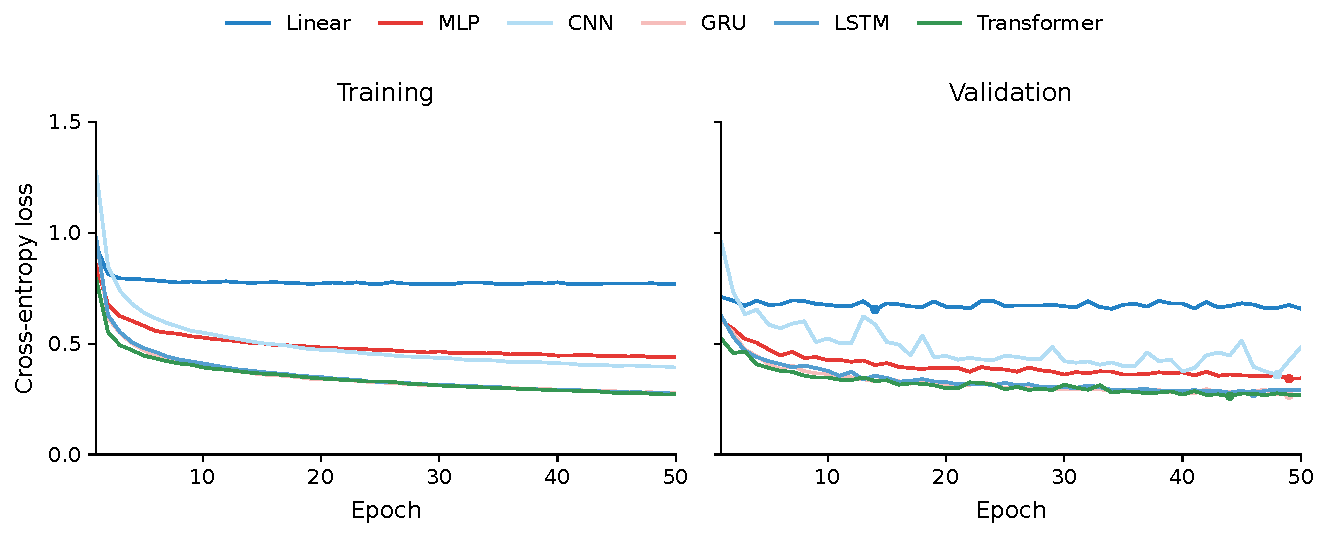
\includegraphics[width=0.88\linewidth]{Images/fashion_mnist_learning.pdf}
\caption{Fashion-MNIST training and validation cross-entropy for six models. Dots mark the selected checkpoints.}
\label{fig:learning-comparison}
\end{figure}

\subsection{Per-class performance and error analysis}
\label{sec:errors}
Confusions among T-shirt/top, Pullover, Coat, and Shirt account for 507 of CNN's
741 errors, or 68.4\%. Here, both the true and predicted labels are in this group.
CNN correctly identifies 79.5\% of Shirt images, compared with 62.1\% for MLP.
It misclassifies 81 Shirt images as T-shirt/top and 61 Coat images as Pullover.
The upper-body classes have similar average shapes in Figure~\ref{fig:class-means},
and they also account for most CNN errors. We have not tested which image details
cause these errors.
\begin{table}[htbp]
\centering\small
\caption[Fashion-MNIST recall by class]{Fashion-MNIST test recall by class, in percent. Each class contains
1,000 test images. All six models use seed 42 and validation-selected
checkpoints from 50-epoch runs.}
\label{tab:class-recall}
\begin{tabular}{lrrrrrr}
\toprule
Class & Linear & MLP & CNN & GRU & LSTM & Transformer\\
\midrule
T-shirt/top & 75.5 & 84.4 & 86.7 & 85.1 & 83.0 & 81.8 \\
Trouser & 90.7 & 97.0 & 96.2 & 97.3 & 98.3 & 98.0 \\
Pullover & 62.8 & 79.8 & 86.3 & 81.6 & 81.6 & 84.0 \\
Dress & 77.0 & 87.5 & 80.3 & 89.5 & 88.7 & 93.2 \\
Coat & 68.1 & 79.7 & 67.8 & 85.4 & 84.6 & 85.6 \\
Sandal & 89.0 & 95.3 & 96.5 & 96.7 & 95.8 & 96.6 \\
Shirt & 40.3 & 62.1 & 59.6 & 72.4 & 70.9 & 72.3 \\
Sneaker & 84.4 & 93.7 & 95.8 & 95.5 & 98.7 & 97.2 \\
Bag & 89.2 & 97.1 & 97.4 & 98.1 & 98.2 & 98.7 \\
Ankle boot & 93.5 & 95.2 & 95.5 & 97.2 & 95.4 & 96.9 \\
\bottomrule
\end{tabular}
\end{table}


CNN's advantage is not uniform across classes. It reaches 99.2\% recall for Bag
and 99.0\% for Trouser, while Shirt remains its weakest class at 79.5\%.
LSTM, on the other hand, has higher Sneaker recall than CNN at 98.7\% versus
97.5\%, and Transformer has slightly higher Dress recall at 93.2\% versus
92.9\%. Overall accuracy therefore hides some class-specific advantages of
the lower-ranked models.

\begin{figure}[H]
\centering
\begin{minipage}[t]{0.49\linewidth}
\centering
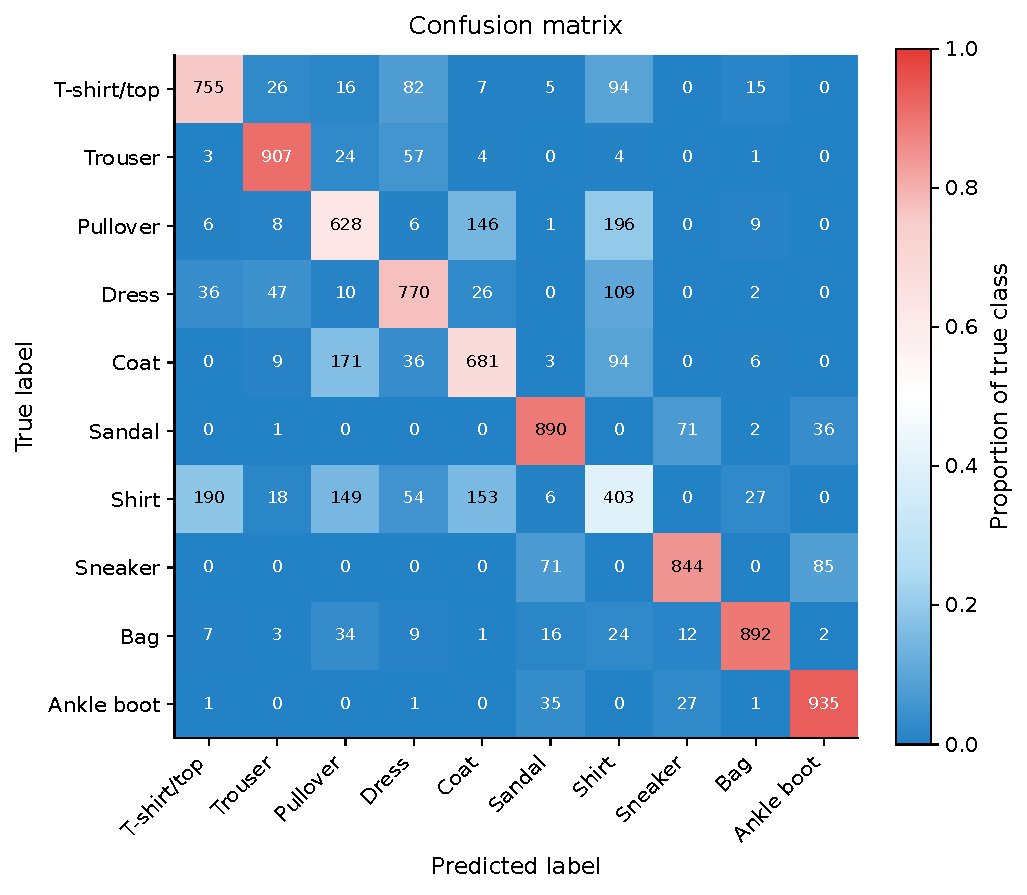
\includegraphics[width=\linewidth]{Images/fashion_mnist_linear_confusion.pdf}
\par\small Linear
\end{minipage}
\hfill
\begin{minipage}[t]{0.49\linewidth}
\centering
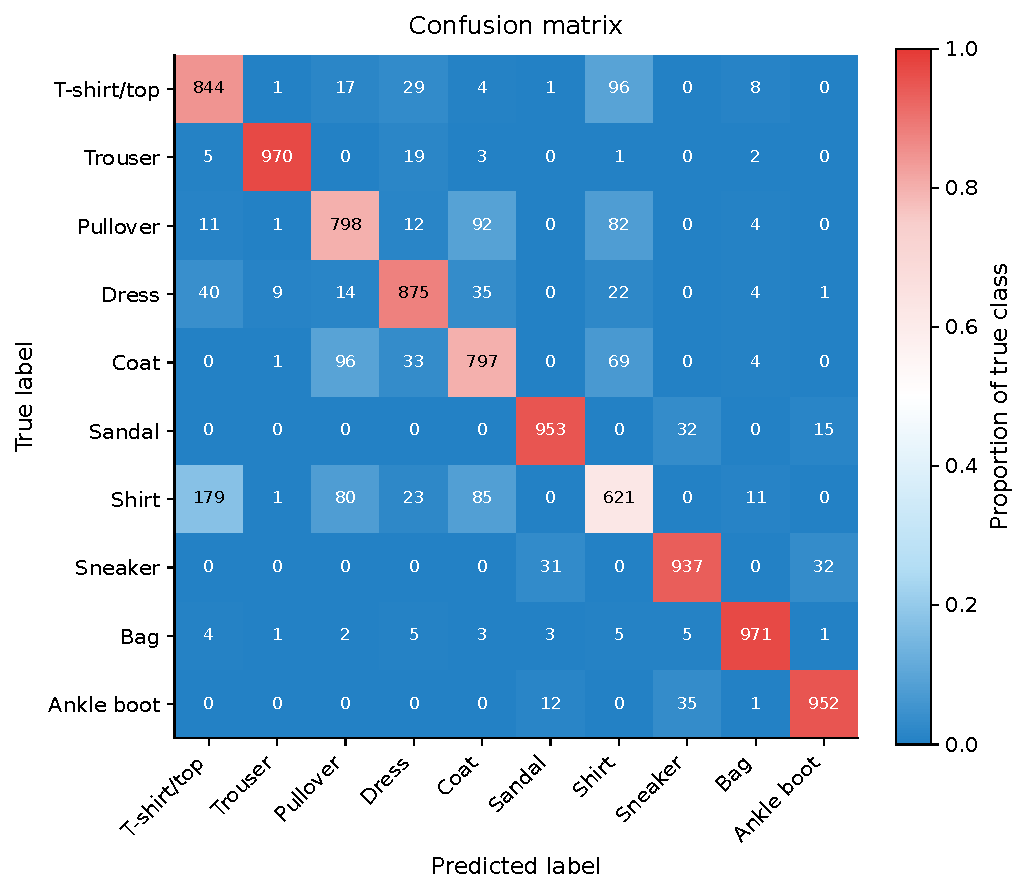
\includegraphics[width=\linewidth]{Images/fashion_mnist_mlp_confusion.pdf}
\par\small MLP
\end{minipage}
\caption{Linear and MLP confusion matrices on the Fashion-MNIST test set. Rows show true classes and columns show predictions. Cell labels give counts, and color gives the fraction of each true class.}
\label{fig:confusion-linear}
\label{fig:confusion-mlp}
\end{figure}

\begin{figure}[H]
\centering
\begin{minipage}[t]{0.49\linewidth}
\centering
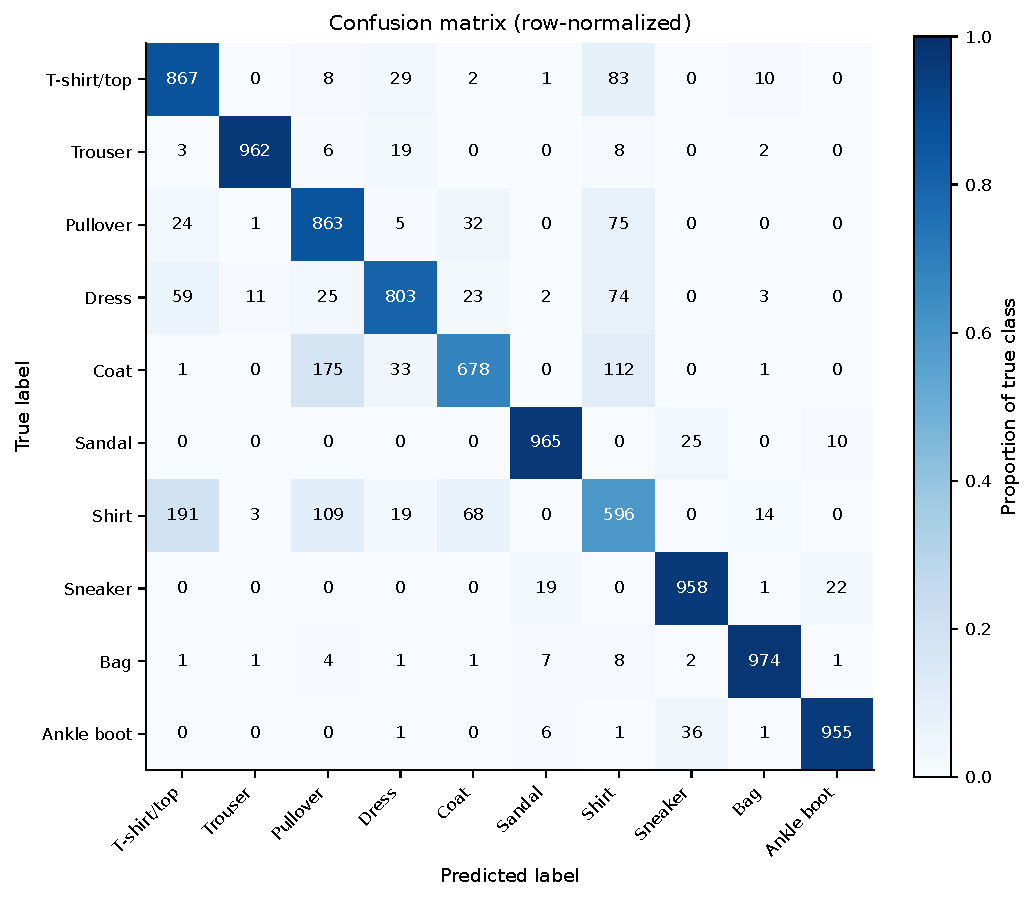
\includegraphics[width=\linewidth]{Images/fashion_mnist_cnn_confusion.pdf}
\par\small CNN
\end{minipage}
\hfill
\begin{minipage}[t]{0.49\linewidth}
\centering
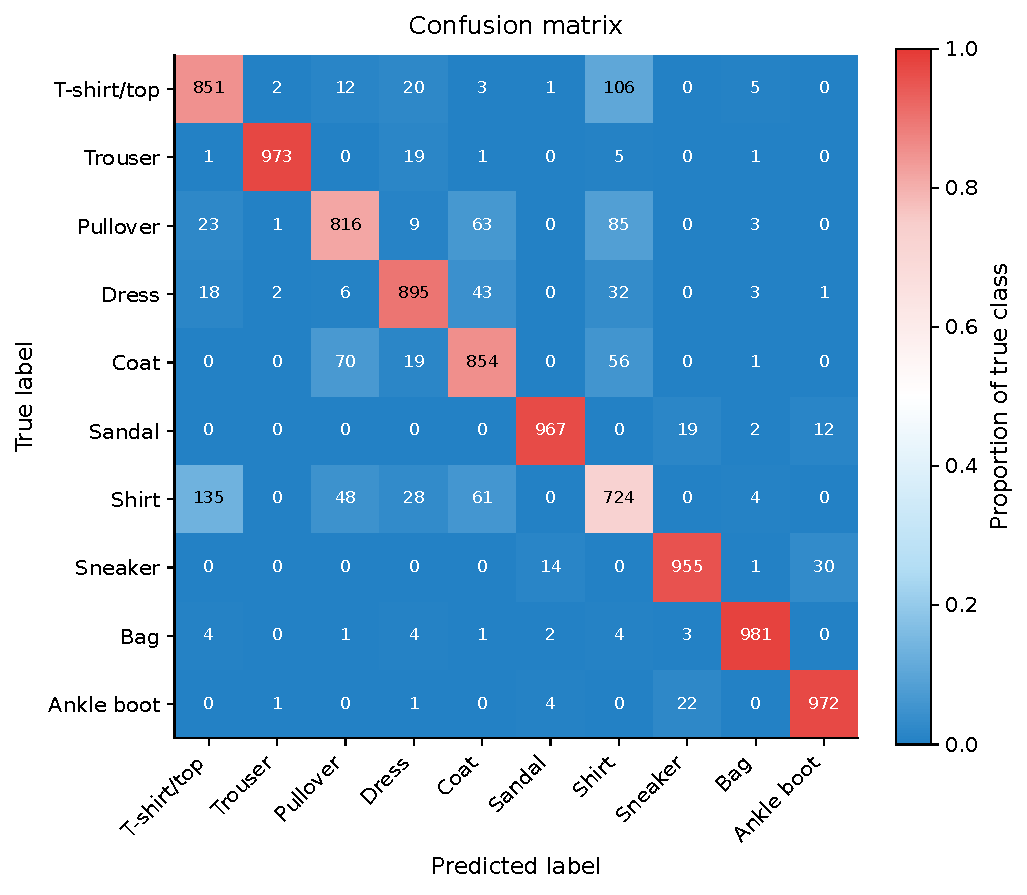
\includegraphics[width=\linewidth]{Images/fashion_mnist_gru_confusion.pdf}
\par\small GRU
\end{minipage}
\caption{CNN and GRU confusion matrices on the Fashion-MNIST test set. Rows show true classes and columns show predictions. Cell labels give counts, and color gives the fraction of each true class.}
\label{fig:confusion-cnn}
\label{fig:confusion-gru}
\end{figure}

\begin{figure}[H]
\centering
\begin{minipage}[t]{0.49\linewidth}
\centering
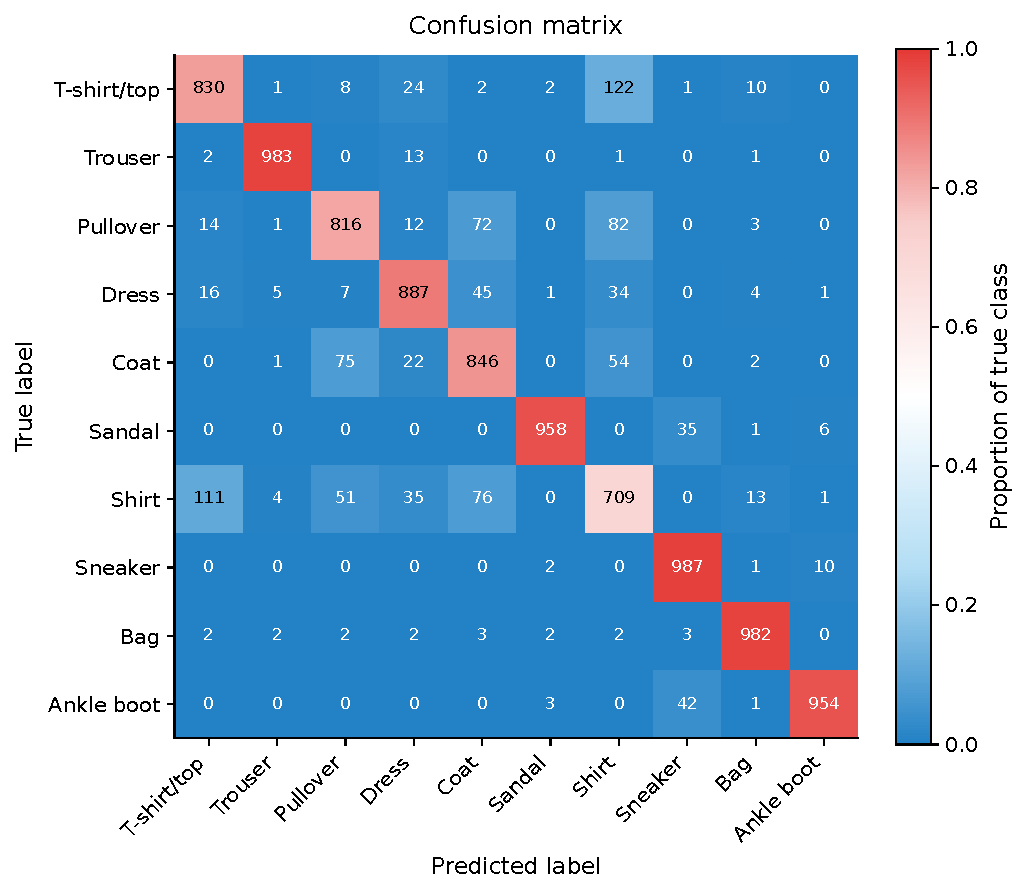
\includegraphics[width=\linewidth]{Images/fashion_mnist_lstm_confusion.pdf}
\par\small LSTM
\end{minipage}
\hfill
\begin{minipage}[t]{0.49\linewidth}
\centering
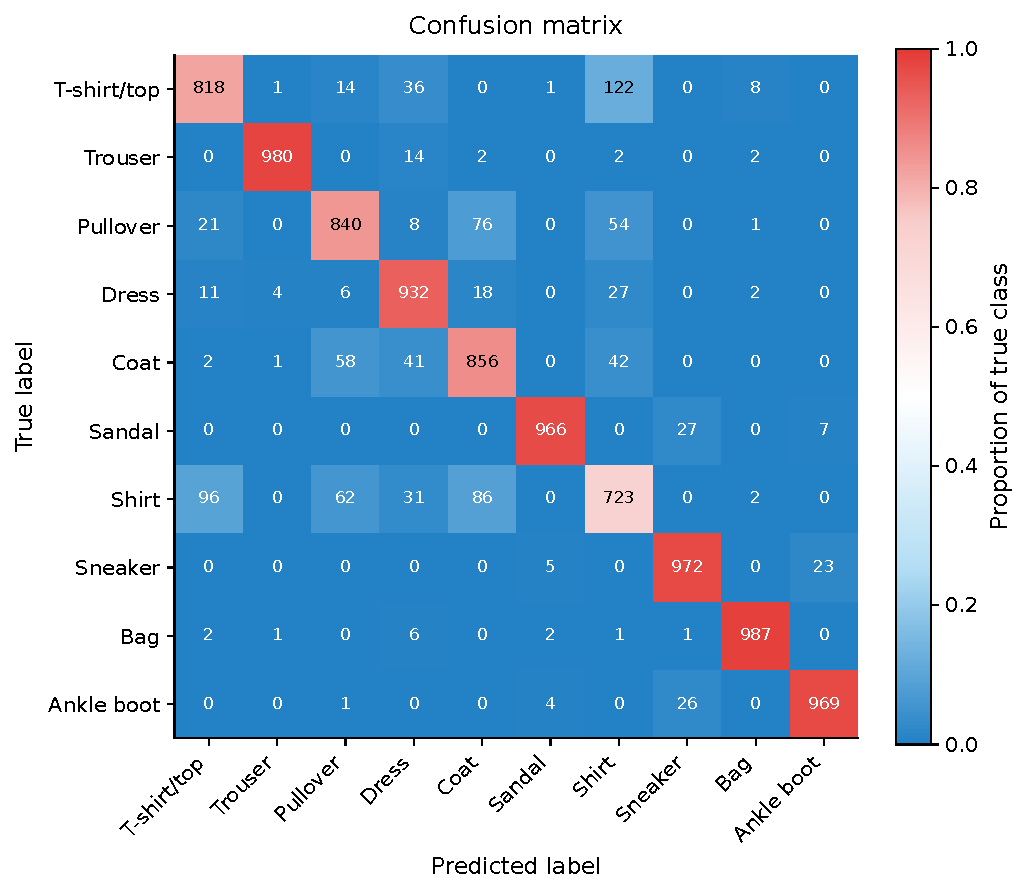
\includegraphics[width=\linewidth]{Images/fashion_mnist_transformer_confusion.pdf}
\par\small Transformer
\end{minipage}
\caption{LSTM and Transformer confusion matrices on the Fashion-MNIST test set. Rows show true classes and columns show predictions. Cell labels give counts, and color gives the fraction of each true class.}
\label{fig:confusion-lstm}
\label{fig:confusion-transformer}
\end{figure}
\subsection{Predictions on shared images}\label{sec:qualitative}
CNN correctly classifies 775 images that MLP misses, while MLP correctly
classifies 234 images that CNN misses. Both models misclassify 507 images and
correctly classify 8,484. These counts distinguish the overall accuracy gain
from a consistent improvement on every image. In particular, the 234 MLP-only
successes identify cases worth inspecting even though CNN performs better on
the full test set.

Figure~\ref{fig:shared-predictions}  shows five models on the same six images.
Each disagreement category has two examples, so the figure does not show how
often each outcome occurs. LSTM is omitted because its per-image predictions
are unavailable for this figure.
\reportfigure{Images/fashion_mnist_shared_images.pdf}{Fashion-MNIST predictions on the first two test images in each category: CNN correct and MLP wrong, both wrong, and MLP correct and CNN wrong. Indices are zero-based. Baseline denotes MLP.}{fig:shared-predictions}

The selected examples show several kinds of disagreement. On test image 25,
which is a Coat, CNN and MLP predict Pullover and Shirt respectively, while
Transformer predicts Coat correctly. On image 23, an Ankle boot, Linear is
correct even though CNN and MLP both predict Sandal. These examples show why a
shared error between the two main models should not automatically be treated
as an unrecognizable image.

\subsection{Limitations}
We use one seed per model and do not run a systematic hyperparameter search or
component ablation, so we cannot assess variation across training runs.
Architecture, model size, and regularization change together, which prevents us
from isolating the effect of each choice. Training and inference times also use
different hardware or measurement conditions. Since inference timings lack
warm-up and repeated trials, we do not compare model speed.

\subsection{Discussion and conclusion}
\label{sec:discussion}
CNN achieves the highest Fashion-MNIST test accuracy at 92.59\%, exceeding the
Transformer by 2.16 percentage points while using 421,738 parameters compared
with 1,191,050. The larger Transformer therefore offers no accuracy advantage
in this experiment. On the other hand, GRU reaches 89.88\% with just 61,962
parameters, making it a smaller alternative when model storage matters more
than the additional 2.71 percentage points achieved by CNN. These results show
why parameter count and accuracy should be considered together when choosing
among the tested models.

One possible explanation for the Transformer result is the amount of training
data relative to what the model must learn from scratch. CNN filters already
connect nearby pixels and share weights across image positions, whereas our
Transformer projects whole rows into tokens and learns relationships between
them through attention. Vision Transformer research links weaker built-in
spatial assumptions to greater data requirements \cite{vit}. Here, the
Transformer learns from 54,000 training images without pretraining, so its
larger capacity does not guarantee better generalization. We did not vary the
training-set size, however, and cannot attribute the accuracy gap to data volume
alone. Data-efficient Transformer training also shows that training strategy
can reduce the need for external data \cite{deit}.

The visual setting also helps explain why convolution is a suitable choice.
Fashion-MNIST images contain isolated products on mostly dark backgrounds,
with fewer distractions than full scenes containing clutter or several objects.
Under these conditions, local edges, sleeves, and garment outlines offer useful
cues for classification, while the benefit of connecting distant image regions
through attention is less obvious. The task still has difficult distinctions.
Confusions among upper-body garments account for 68.4\% of CNN errors, so a
simple background does not make Shirt, Coat, and Pullover easy to separate.

For this dataset and training setup, CNN is the strongest tested choice for
accuracy, while GRU provides a smaller model with a moderate accuracy cost.
The Transformer is not a better alternative under the current protocol, but
this result does not rule out improvements from pretraining, different image
tokens, or a training schedule designed for Transformers. MLP also correctly
classifies 234 images that CNN misses, showing that the best overall model still
has individual failures. A useful follow-up would vary training-set size for
both CNN and Transformer under fixed settings and repeat the runs across seeds.
This would test the data-size explanation directly rather than infer it from
one accuracy comparison.
